\documentclass{article}
\usepackage[utf8]{inputenc}
\usepackage{graphicx}
\usepackage{verbatim}

\vspace{\stretch{1}}

\title{\LARGE Applicativo Java per la gestione di un ristorante \\
\large Elaborato Ingegneria del Software}
\author{Gianni Moretti, Francesco Fantechi, Francesco Bettazzi}
\date{A.A. 2020-2021}

\begin{document}

\maketitle

\begin{figure}[!h]
\centering
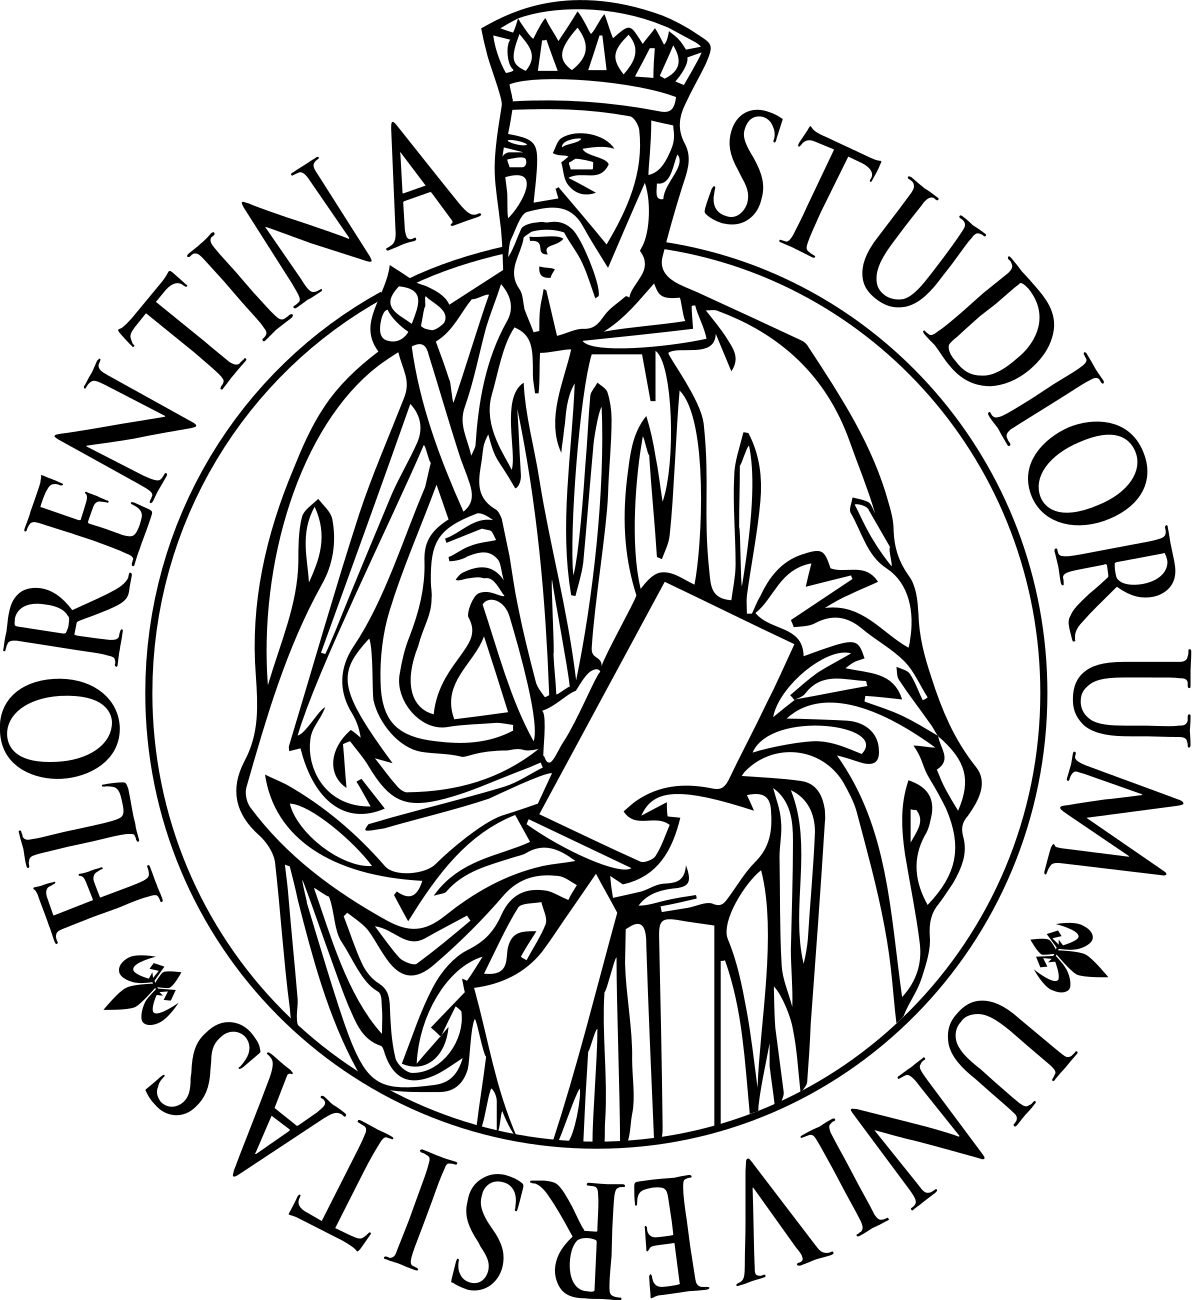
\includegraphics[width=4cm, height=4cm]{"Immagini/LogoUnifi.PNG"}
\end{figure}

\begin{center}
\textbf{\large UNIVERSITA' DEGLI STUDI DI FIRENZE \\
Facolta di Ingegneria \\
\normalsize Corso di Laurea in Ingegneria Informatica}
\end{center}

\vspace{\stretch{1}}

\newpage

% Indice
\tableofcontents

\newpage

\section{Motivazione e Descrizione}
Il presente elaborato nasce dall'idea di uno di noi ragazzi che, lavorando in una pizzeria come cameriere, si \`e trovato ad interagire con un applicativo simile. Abbiamo cos\`i pensato di riprodurne uno personalizzato che preveda inoltre, considerato il periodo particolare che stiamo vivendo, la possibilit\`a di gestire azioni atte alla sicurezza dei clienti, come il loro monitoraggio per poterli rintracciare. \\
L'applicativo ha lo scopo di gestire le varie parti che compongono un ristorante, in modo da farle interagire e collaborare assieme. Abbiamo individuato le cinque figure professionali principali che possono trovarsi ad agire all'interno di un ristorante:

\begin{enumerate}
\item L'organizzatore della sala: \`e colui che all'arrivo di nuovi clienti ha il compito di assegnare loro un tavolo. Ci\`o pu\`o essere realizzato utilizzando i tavoli singoli gi\`a disposti in sala ad inizio serata o aggregandone alcuni se il numero di clienti \`e  elevato. Ha quindi la possibilit\`a di contrassegnare come occupati i tavoli assegnati e di rimetterli disponibili una volta terminato il servizio e igienizzato il tavolo. Inoltre, in vista delle norme di distanziamento imposte dal periodo che stiamo vivendo, l'organizzatore della sala pu\`o decidere se e quali tavoli sono o no utilizzabili. 
\item Il cameriere: ha il compito di gestire i vari servizi ai tavoli, ossia di prendere le comande e mandarle alla cucina per la loro realizzazione. Le comande sono composte da un insieme di piatti presenti nel men\`u del locale, da dei commenti opzionali sui piatti per la cucina e da un insieme di ingredienti aggiunti/rimossi dalle varie portate su preferenza e richiesta del cliente. In caso di  errore di immissione della comanda o di richiesta di modifica da parte del cliente, il cameriere pu\`o eliminare le portate sbagliate in modo da correggere correttamente il conto. Per aprire un servizio al tavolo il cameriere \`e tenuto a prendere un nominativo ed un recapito telefonico di uno dei presenti in modo da tenere traccia di chi ha frequentato il locale ed essere in grado di rintracciare i clienti in caso di necessit\`a. 
\item La cucina: i cuochi ottengono le comande confermate dai camerieri e possono spuntarle una volta preparate le pietanze. La cucina si pu\`o inoltre specializzare in pi\`u aree di competenza come, ad esempio, la pizzeria e il bar. 
\item Il cassiere: \`e colui che al termine del servizio a un tavolo esegue il conto, contrassegna il tavolo come da pulire ed igienizzare e si occupa di memorizzare correttamente i dati dei clienti presenti.
\item Il gestore del ristorante: \`e colui che ha accesso ai dati memorizzati dei clienti. Pu\`o inoltre modificare il men\`u del locale aggiungendo portate e variando gli ingredienti in esse presenti, al fine, per esempio, di aggiungere una specialit\`a del giorno.
\end{enumerate}

\subsection{Possibili aggiunte}

Nonostante non siano state implementate, riportiamo di seguito delle possibili aggiunte per il nostro applicativo:

\begin{itemize}
\item Ordini a domicilio o da asporto
\item Prenotazioni dei tavoli
\item Login dei vari dipendenti
\end{itemize}

\subsubsection{Ordini a domicilio o da asporto}
L'applicazione potrebbe consentire di effettuare ordini da casa attraverso un sistema di consegna a domicilio oppure per l'asporto. Gli ordini verrebbero aggiunti direttamente all' ``OrderManager" che provvederebbe a smistarli alle cucine. Al fine di diversificare gli ordini fatti da casa da quelli presi ai tavoli, emergerebbe la necessit\`a di un nuovo attributo alla classe ``Order" denominato ``takeAway". In base al valore di questo attributo le cucine saprebbero come gestire gli ordini.  

\subsubsection{Prenotazioni dei tavoli}  
L'organizzatore della sala potrebbe gestire le prenotazioni fatte dai clienti. Questo \`e realizzabile attraverso un database contenente le prenotazioni ricevute. L'orga-\\nizzatore della sala avrebbe la possibilit\`a di scrivere e leggere le prenotazioni relative ad una certa data al fine di poter organizzare la sala di conseguenza.

\subsubsection{Login dei vari dipendenti}
Al momento del login i dati inseriti verrebbero confrontati con quelli presenti all'interno di un database. Solo se i dati trovano una corrispondenza l'applicazione consentirebbe di accedere alla pagina richiesta. Il manager del ristorante sarebbe in grado di aggiungere e rimuovere le credenziali dei vari dipendenti a sua discrezione per regolamentare i ruoli.

\newpage

\section{Requisiti}
\subsection{Use Case}

Dalla descrizione del nostro modello di dominio abbiamo identificato gli attori in gioco con le varie figure professionali del ristorante e i rispettivi casi d'uso con le rispettive mansioni. Di seguito viene riportato l'Use Case Diagram risultante:

\begin{figure}[!h]
\centering
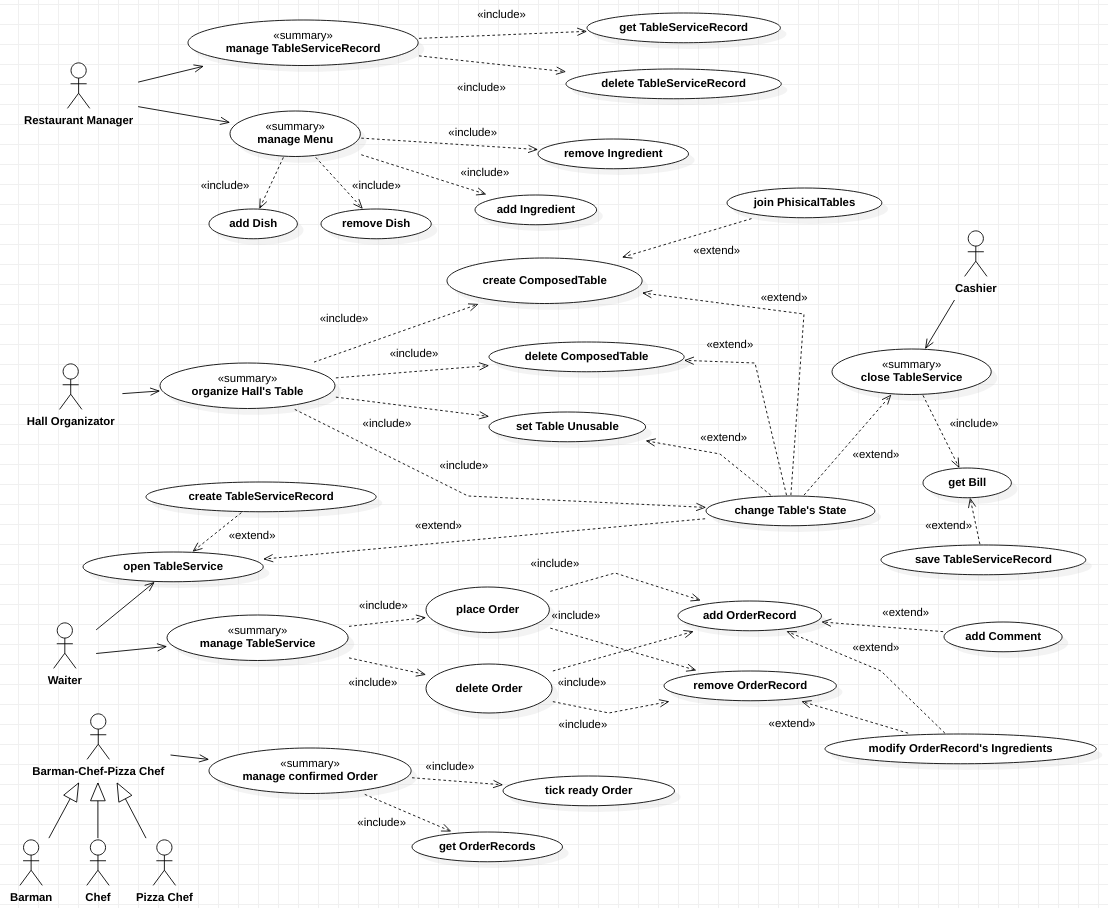
\includegraphics[width= 15cm]{"Immagini/UseCaseDiagram.PNG"}
\caption{Use Case Diagram}
\end{figure}

\newpage

\subsection{Use Case Template}
Riportiamo di seguito i template relativi ad alcuni dei pricipali casi d'uso individuati nel nostro progetto:

\begin{figure}[!h]
\centering
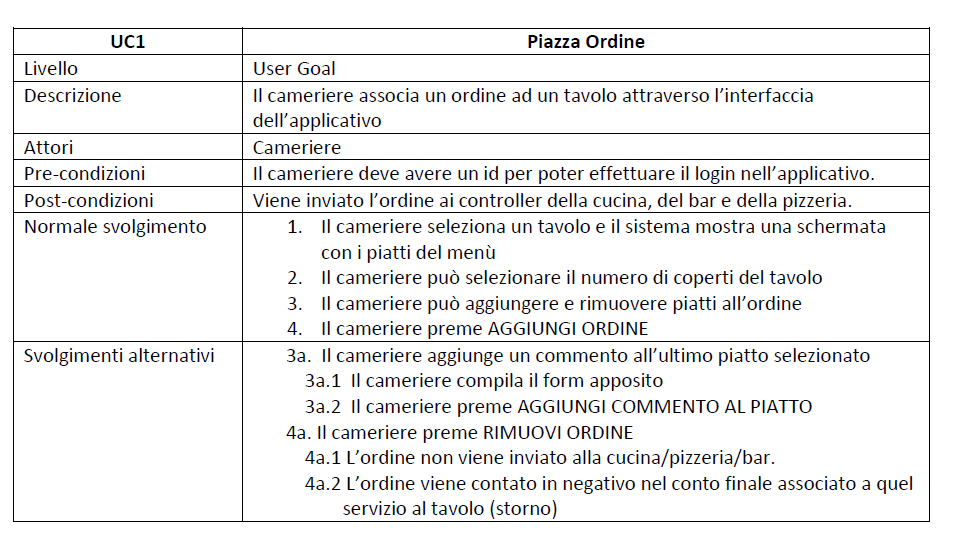
\includegraphics[width= 10cm]{"Immagini/PlaceOrder.PNG"}
\caption{Template che descrive il caso d'uso del cameriere per piazzare un ordine ad un servizio al tavolo}
\end{figure}

\begin{figure}[!h]
\centering
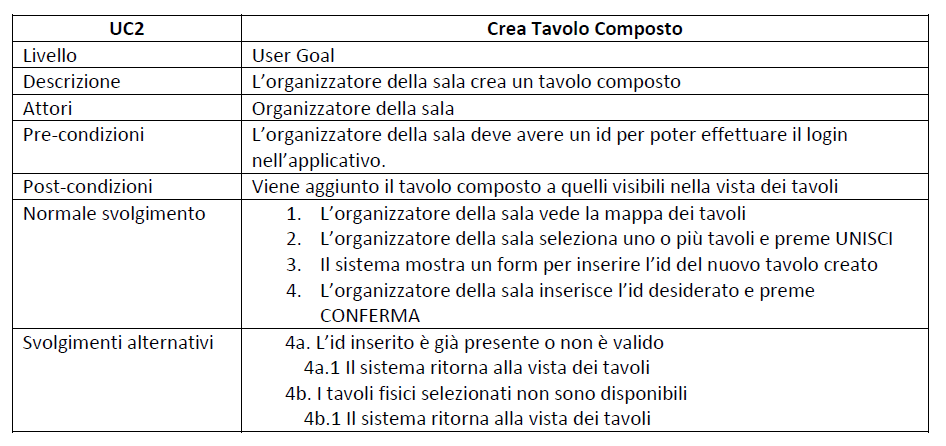
\includegraphics[width= 10cm]{"Immagini/CreateComposedTable.PNG"}
\caption{Template che descrive il caso d'uso dell'organizzatore della sala per creare un tavolo composto}
\end{figure}

\newpage

\begin{figure}[!h]
\centering
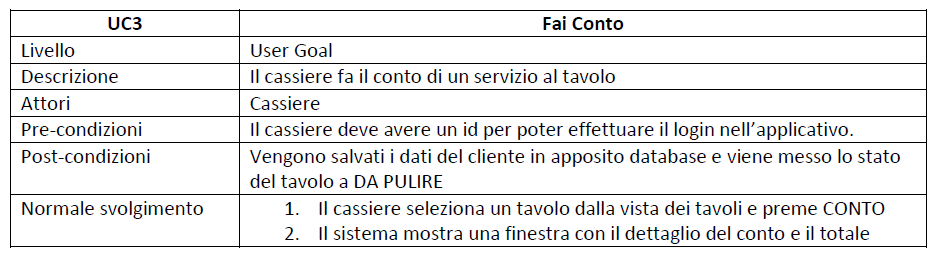
\includegraphics[width= 10cm]{"Immagini/GetBill.PNG"}
\caption{Template che descrive il caso d'uso del cassiere per calcolare il conto di un servizio al tavolo}
\end{figure}

\subsection{Mockups}
Riportiamo di seguito dei possibili mockups relativi alle interfaccie grafiche della nostra app per l'interazione con i nostri attori.

\begin{figure}[!h]
\centering
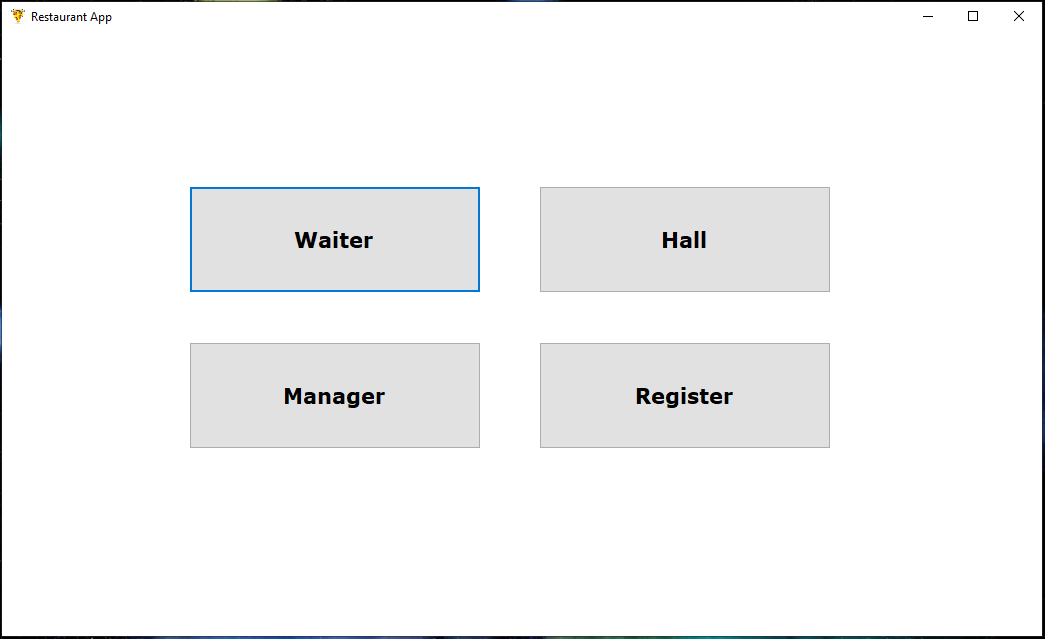
\includegraphics[width= 10cm]{"Immagini/HomePage.PNG"}
\caption{Mockup raffigurante un prototipo della home page dell'app}
\end{figure}

\newpage

\begin{figure}[!h]
\centering
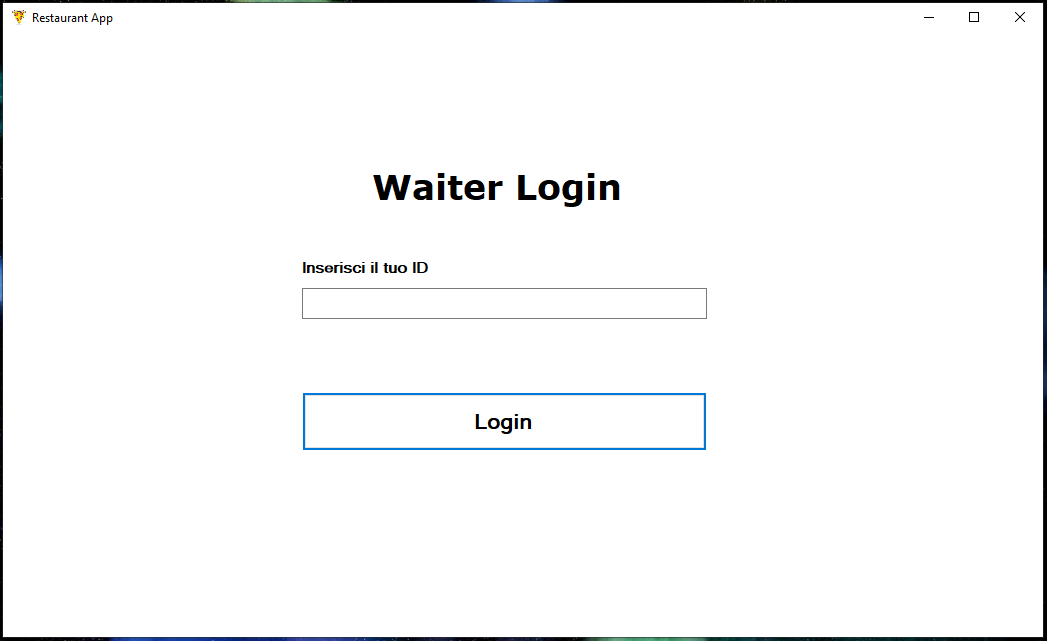
\includegraphics[width= 10cm]{"Immagini/WaiterLogin.PNG"}
\caption{Mockup raffigurante un prototipo della pagina di login del cameriere}
\end{figure}

\begin{figure}[!h]
\centering
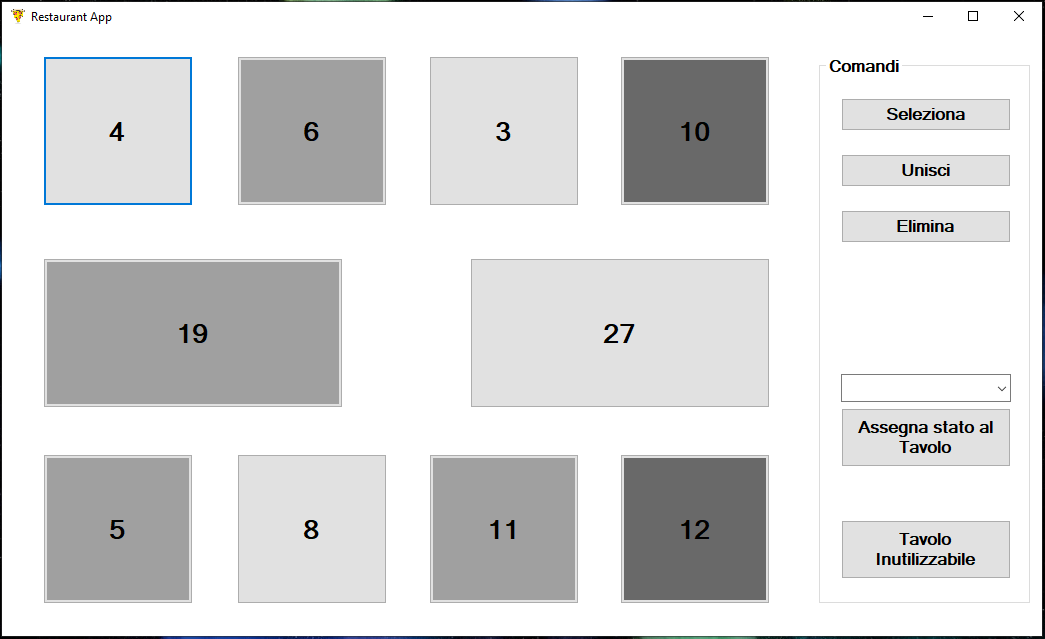
\includegraphics[width= 10cm]{"Immagini/HallOrganizatorPage.PNG"}
\caption{Mockup raffigurante un prototipo dell'interfaccia dell'organizzatore della sala}
\end{figure}

\newpage

\begin{figure}[!h]
\centering
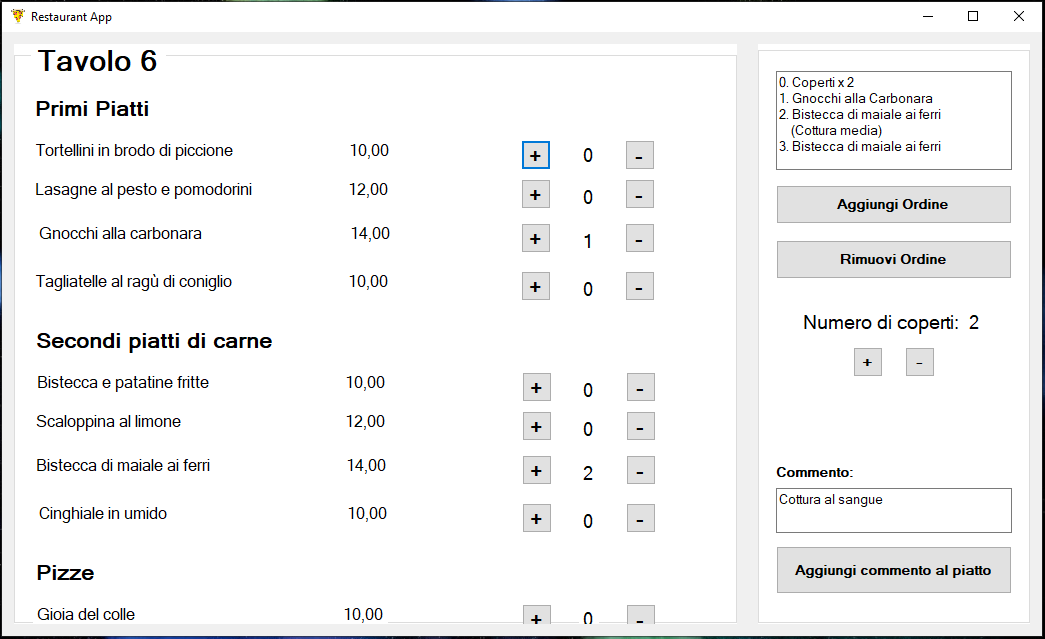
\includegraphics[width= 10cm]{"Immagini/OrdineCameriere.PNG"}
\caption{Mockup raffigurante un prototipo dell'interfaccia del cameriere al momento della creazione di un ordine}
\end{figure}

\section{Progettazione e Implementazione}
\subsection{Scelte implementative e considerazioni}
Per implementare il nostro progetto in linguaggio Java ed eseguire i test ci siamo serviti dell'IDE Eclipse. Al fine di semplificare la collaborazione abbiamo utilizzato GitHub come stumento di versionamento del codice. Per quanto riguarda il Class Diagram, l'Use Case Diagram, il Sequance Diagram e lo schema architetturale in packages ci siamo serviti del software StarUML. \\
Per le competenze richieste dall'elaborato, lo schema da noi riportato e implementato ha il solo scopo di illustrare le interazioni principali fra le varie parti, non \`e quindi atto ad una realizzazione concreta. L'applicativo si presta, infatti, per essere realizzato ad operare come un sistema distribuito, prevedendo cio\`e un server centrale con al suo interno dati comuni accessibili dai vari terminali attraverso un protocollo di comunicazione.
Ad esempio, l'applicativo in esecuzione sul tablet del cameriere mostrerebbe l'interfaccia collegata al WaiterPageController che dialogherebbe con un server tramite delle classi che permettono tale comunicazione. In questo modo il client cameriere sarebbe in grado di aggiungere dei ``TableService" al ``TableServiceContainer" che si troverebbe all'interno del server comune.  

\newpage

\subsection{Class Diagram}
Qui di seguito riportiamo la realizzazione del Class Diagram che descrive la nostra logica di dominio in prospettiva di implementazione:

\begin{figure}[!h]
\centering
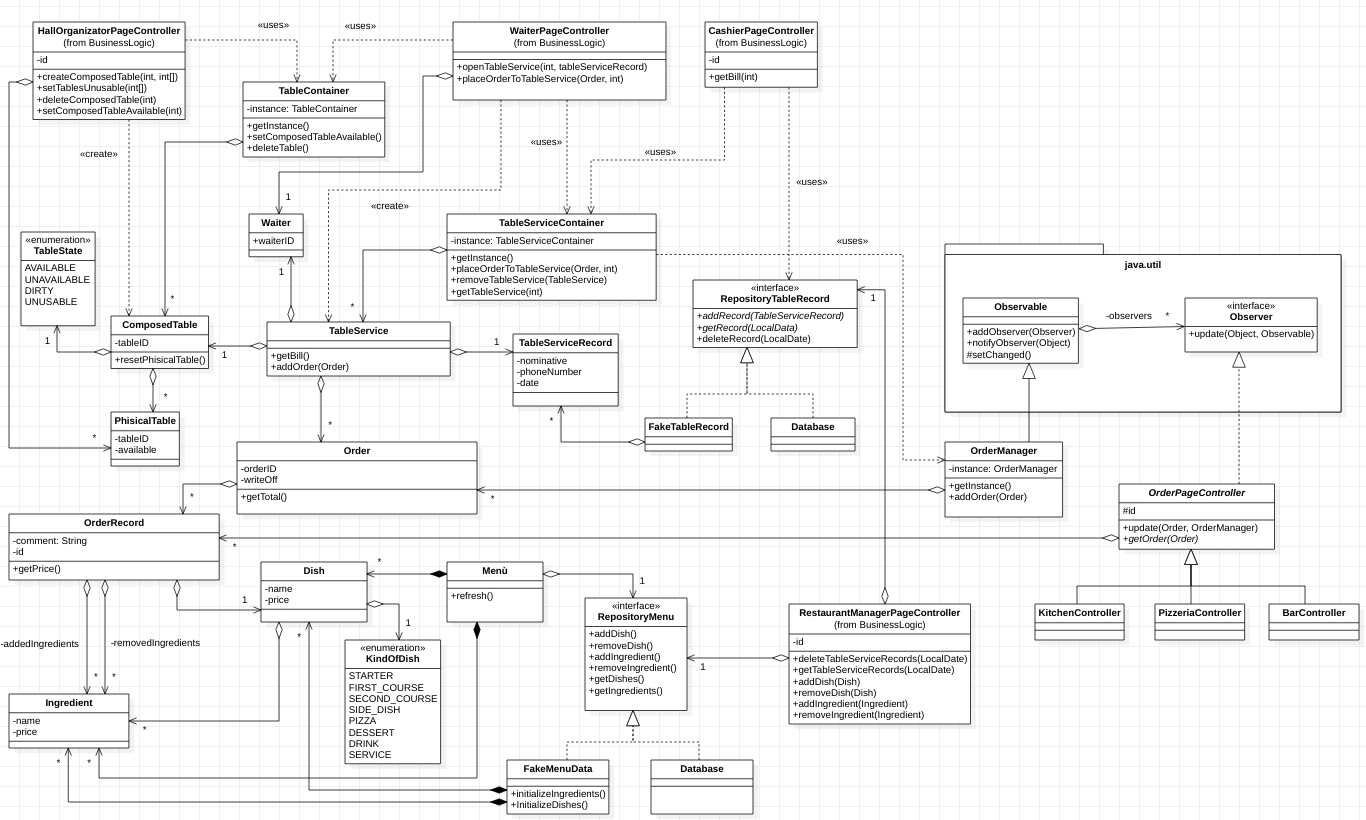
\includegraphics[width= 15cm]{"Immagini/ClassDiagram.PNG"}
\caption{Class Diagram}
\label{ClassDiagram}
\end{figure}

\newpage

\subsection{Classi ed Interfacce}
Per l'implementazione del nostro applicativo abbiamo sia definito nuove classi ed interfacce specifiche, sia utilizzato alcune di quelle gi\`a presenti nelle librerie standard di Java. \\
Le classi Controller sotto riportate vengono create al momento del login di un client nella relativa interfaccia grafica, sono una per ciascun attore e vengono utilizzate nei seguenti modi: 

\subsubsection{WaiterPageController}

Tramite questo controller, il cameriere pu\`o inserire nuovi ordini relativi ad un determinato tavolo utilizzando il metodo \textit{placeOrderToTableService()}, oppure creare un nuovo TableService con il metodo \textit{openTableService()} indicando il tavolo interessato.

\begin{figure}[!h]
\centering
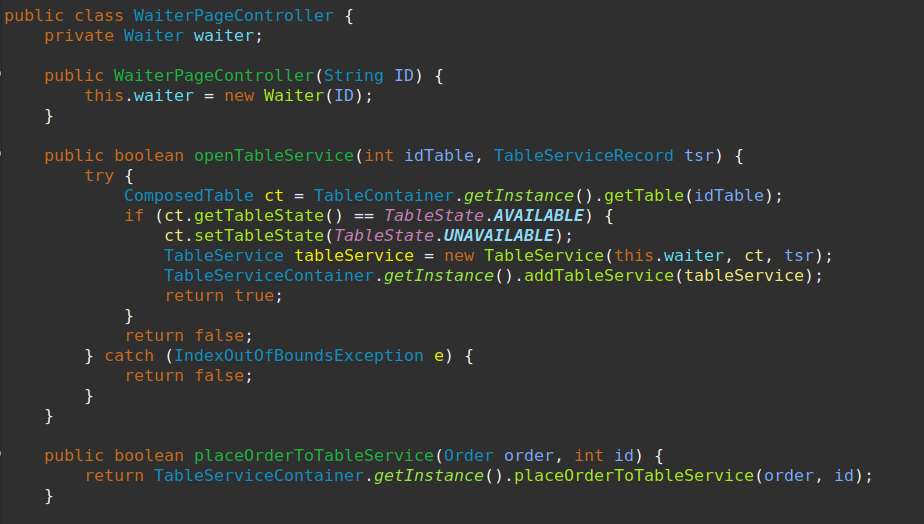
\includegraphics[width= 12cm]{"Codice/WaiterPageController.PNG"}
\caption{Porzione di codice della classe WaiterPageController}
\end{figure}


\subsubsection{HallOraganizatorPageController}

\`E un controller che permette di organizzare i tavoli presenti nella sala. Al suo interno contiene la lista di tavoli fisici. \`E possibile creare nuovi tavoli composti attraverso il metodo  \textit{createComposedTable()} specificando gli id dei tavoli fisici da utilizzare. Il tavolo composto creato viene direttamente inserito all'interno del ``TableContainer''.
\textit{setTablesUnusable()} ci permette invece di impostare lo stato dei tavoli, specificati con id, nello stato ``Unusable''.

\begin{figure}[!h]
\centering
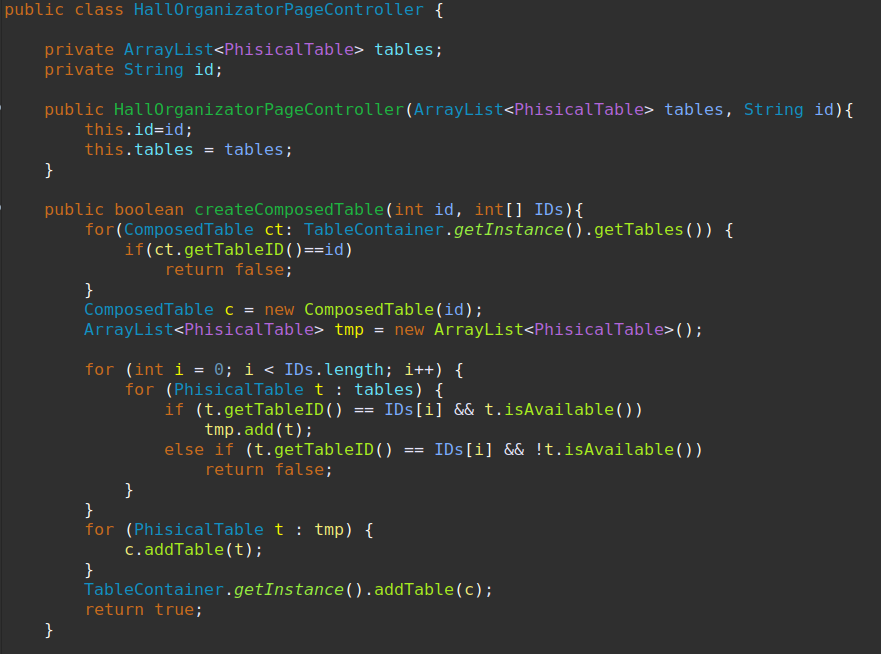
\includegraphics[width= 12cm]{"Codice/HallPage1.PNG"}
\caption{Porzione di codice della classe HallOrganizatorPageController}
\end{figure}

\begin{figure}[!h]
\centering
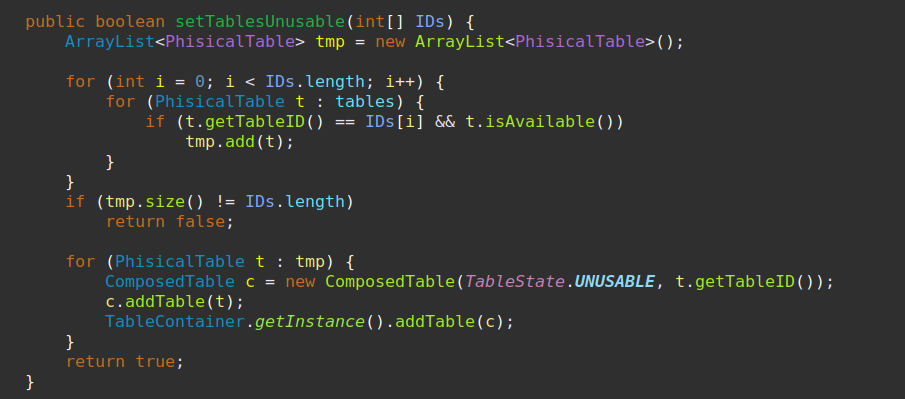
\includegraphics[width= 12cm]{"Codice/HallPage2.PNG"}
\caption{Porzione di codice della classe HallOrganizatorPageController}
\end{figure}

\newpage

\subsubsection{CashierPageController}

Questo controller viene utilizzato dall'interfaccia del cassiere per calcolare il conto relativo ad un servizio al tavolo utilizzando \textit{getBill()}.

\begin{figure}[!h]
\centering
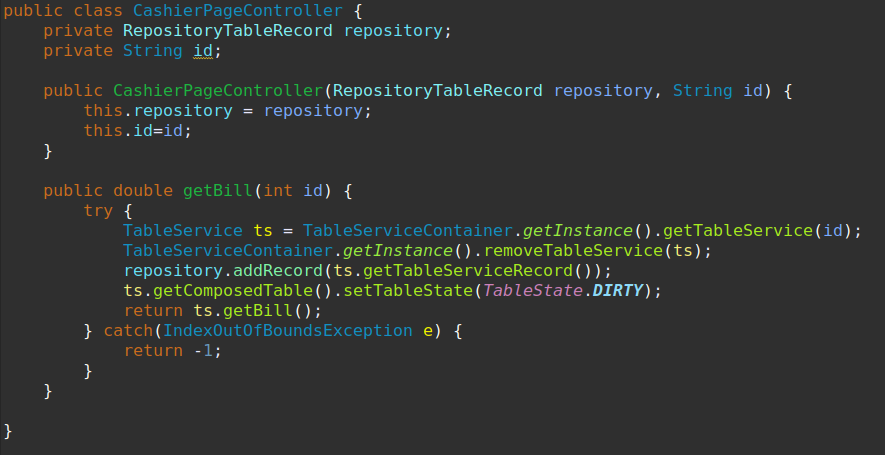
\includegraphics[width= 12cm]{"Codice/CassierePage.PNG"}
\caption{Porzione di codice della classe CashierPageController}
\end{figure}

\newpage

\subsubsection{RestaurantManagerPageController}

Viene utilizzato per la gestione del ``Men\`u'' e dei ``TableServiceRecord'' da parte del manager del ristorante. Al suo interno sono presenti metodi per la gestione del men\`u, ad esempio \textit{addDish()} e \textit{removeDish()} per aggiungere e rimuovere un piatto rispettivamente. Inoltre il manager del ristorante ha la possibilit\`a di cancellare dei ``TableServiceRecord'' relativi ad una data con \textit{deleteTableServiceRecords()} o di visionarli con \textit{getTableServiceRecords()}.

\begin{figure}[!h]
\centering
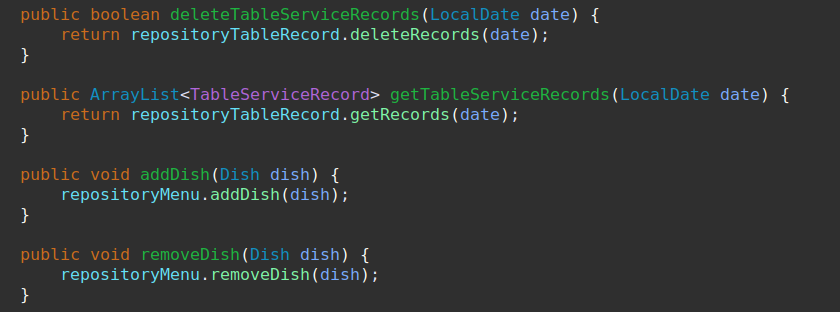
\includegraphics[width= 12cm]{"Codice/ManagerPage.PNG"}
\caption{Porzione di codice della classe RestaurantManagerPageController}
\end{figure}

\newpage


\subsubsection{OrderPageController, BarController, KitchenController e PizzeriaController}

``OrderPageController'' \`e una classe astratta che abbiamo creato per definire i metodi necessari ai controller specifici della cucina: ``BarController'', ``KitchenController'' e ``PizzeriaController''. Questi ultimi, infatti, la implementano e definiscono al loro interno il metodo astratto \textit{getOrder()} in modo tale da prendere soltanto gli ``OrderRecord'' a cui sono interessati. Inoltre ``OrderPageController'' implementa l'interfaccia ``Observer'' del package java.util cos\`i da poter essere avvisata dall' ``OrderManager'' (``Observable'') quando vengono piazzati nuovi ordini e tramite il metodo \textit{update()} aggiornare automaticamente la lista dei suoi ``OrderRecord'' (Vedi Sezione Observer \ref{Observer}).

\begin{figure}[!h]
\centering
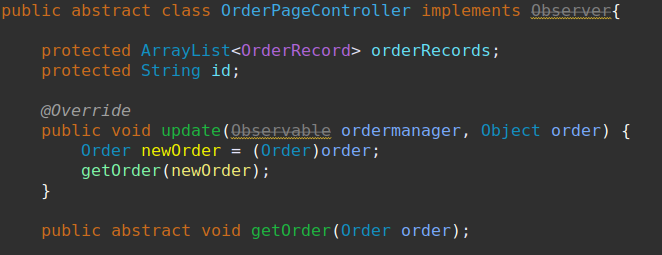
\includegraphics[width= 12cm]{"Codice/OrderPage.PNG"}
\caption{Porzione di codice della classe OrderPageController}
\end{figure}

\begin{figure}[!h]
\centering
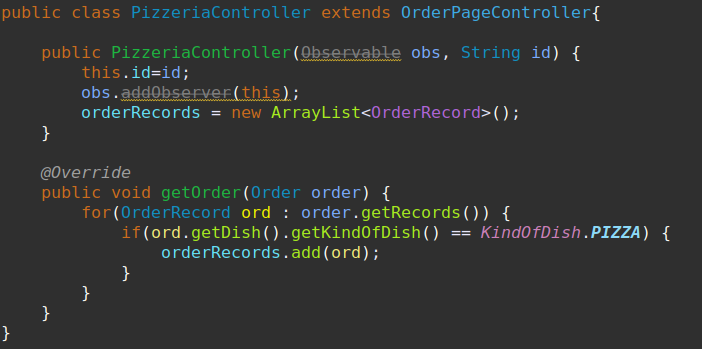
\includegraphics[width= 12cm]{"Codice/PizzeriaPage.PNG"}
\caption{Porzione di codice della classe PizzeriaController}
\end{figure}

\newpage

\noindent Di seguito riportiamo la descrizione di alcune delle classi principali appartenenti alla parte di Domain Model del nostro progetto: 

\subsubsection{PhisicalTable e ComposedTable}

I ``PhisicalTable'' rappresentano i tavoli presenti all'interno del locale, vengono identificati tramite un id e \textit{setAvailable()} permette di renderli utilizzabili o non utilizzabili.

\begin{figure}[!h]
\centering
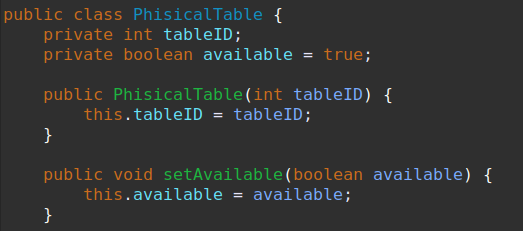
\includegraphics[width= 9cm]{"Codice/PhisicalTable.PNG"}
\caption{Porzione di codice della classe PhisicalTable}
\end{figure}


\noindent ``ComposedTable'' \`e un tavolo composto da un insieme di ``PhisicalTable'' e viene identificato, anche lui, con un id. Il metodo \textit{addTable()} permette di aggiungere un ``PhisicalTable'' al suo interno. Inoltre, \`e possibile assegnargli un ``TableState'' per contrassegnare lo stato in cui si trova.

\begin{figure}[!h]
\centering
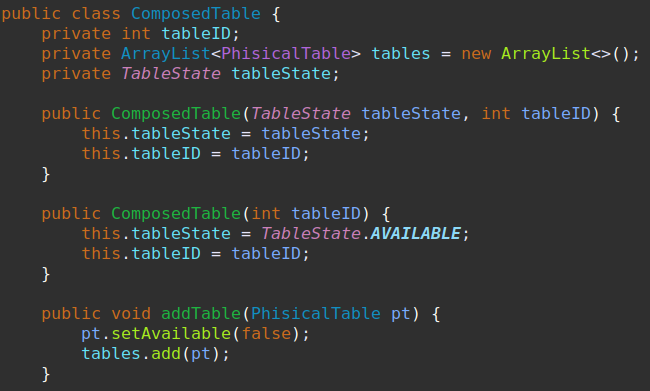
\includegraphics[width= 12cm]{"Codice/ComposedTable.PNG"}
\caption{Porzione di codice della classe Composed}
\end{figure}

\subsubsection{TableContainer}

Contiene tutti i ``ComposedTable'' creati dall'organizzatore della sala in una lista al suo interno. Permette di aggiungere, eliminare o cambiare lo stato ai tavoli composti con i metodi \textit{addTable()}, \textit{deleteTable(int id)} e \textit{setComposedTableAvailable()}.

\begin{figure}[!h]
\centering
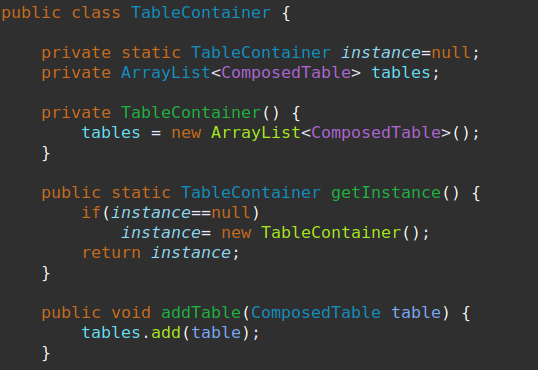
\includegraphics[width= 7cm]{"Codice/TableContainer1.PNG"}
\caption{Porzione di codice della classe TableContainer}
\end{figure}


\begin{figure}[!h]
\centering
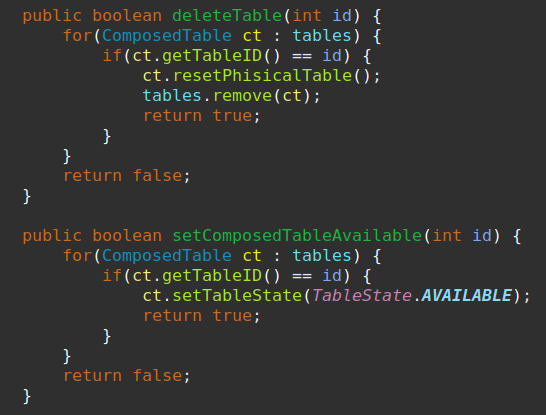
\includegraphics[width= 7cm]{"Codice/TableContainer2.PNG"}
\caption{Porzione di codice della classe TableContainer}
\end{figure}

\newpage

\subsubsection{TableService}

``TableService'' \`e una classe che raggruppa al suo interno tutte le informazioni inerenti al servizio di un tavolo. Al suo interno troviamo infatti: lista degli ordini piazzati, ``TableServiceRecord'', il ``ComposedTable'' a cui \`e associato e il cameriere che lo ha creato e sta effettuando il servizio.


\begin{figure}[!h]
\centering
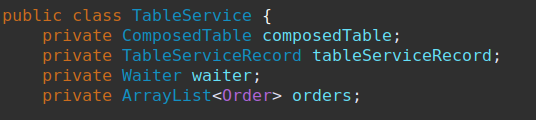
\includegraphics[width= 9cm]{"Codice/TableService.PNG"}
\caption{Porzione di codice della classe TableService}
\end{figure}

\subsubsection{TableServiceContainer}

Contiene tutti i ``TableService'' creati dai camerieri. Permette di gestire i ``TableService'' contenuti al suo interno con diversi metodi come, ad esempio, \textit{addTableService()} per aggiungere un TableService o \textit{placeOrderToTableService()} per aggiungere un ordine al TableService del tavolo id.

\begin{figure}[!h]
\centering
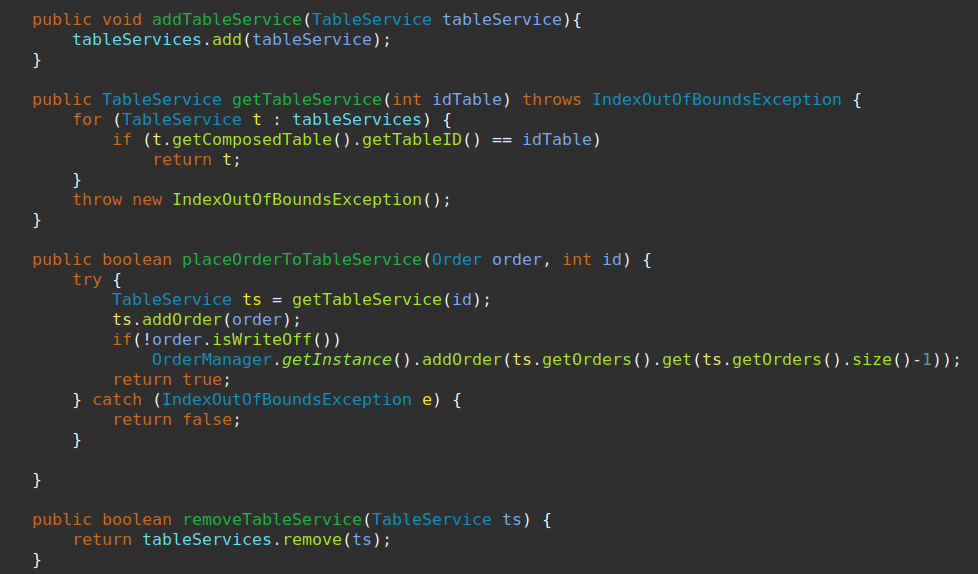
\includegraphics[width= 14cm]{"Codice/TableServiceContainer.PNG"}
\caption{Porzione di codice della classe TableServiceContainer}
\end{figure}

\newpage

\subsubsection{OrderRecord}

Questa classe viene utilizzata per inserire i piatti del men\`u nelle comande e, inoltre, rende possibile l'aggiunta di un commento o la rimozione/aggiunta di ingredienti al piatto. All'interno si trovano infatti due liste di ``Ingredients'', una contenente gli ingredienti aggiunti ``ArrayList$<$Ingredient$>$ addedIngredients'' e l'altra gli ingredienti rimossi ``ArrayList$<$Ingredient$>$  removedIngredients''. Attraverso il metodo \textit{getPrice()} calcola il prezzo del piatto corrispondente sommando e sottraendo il prezzo degli ingredienti rispettivamente aggiunti e rimossi. Ogni ``OrderRecord'' \`e identificato da un id, lo stesso dell' ``Order'' che lo contiene.


\begin{figure}[!h]
\centering
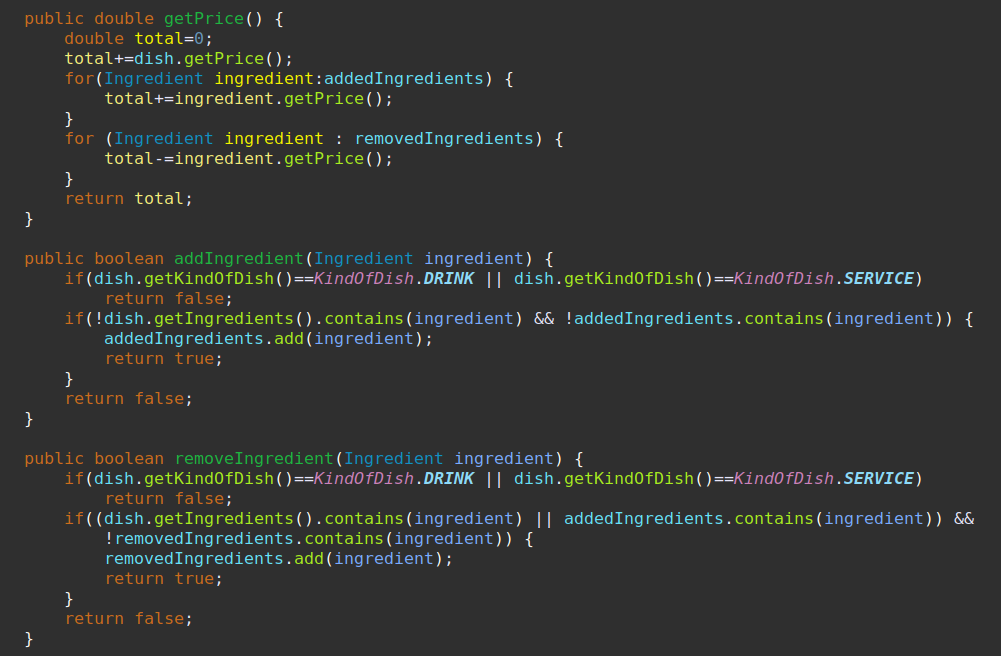
\includegraphics[width= 14cm]{"Codice/OrderRecord.PNG"}
\caption{Porzione di codice della classe OrderRecord}
\end{figure}

\subsubsection{OrderManager}

Si occupa della gestione degli ordini. Al suo interno \`e presente una lista di ordini e con il metodo \textit{addOrder()} se ne possono aggiungere di nuovi. ``OrderManager'' estende la classe astratta ``Observable'' del package java.util, cos\`i che ogni qualvolta venga aggiunto un nuovo ``Order'' alla lista venga richiamato \textit{notifyObservers()} che avvisa gli ``Observer'' (``OrderPageController'') del nuovo ordine aggiunto (Vedi Sezione Observer \ref{Observer}). 

\newpage

\begin{figure}[!h]
\centering
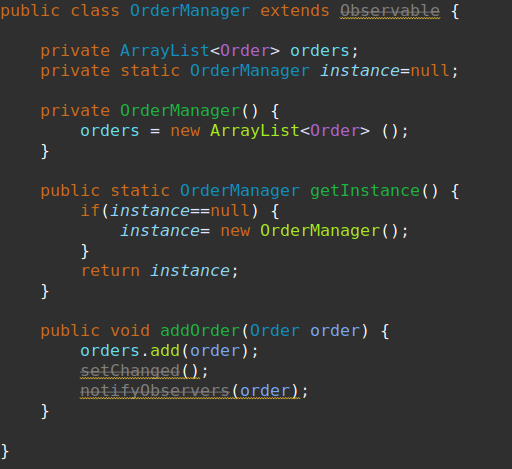
\includegraphics[width= 7.5cm]{"Codice/OrderManager.PNG"}
\caption{Porzione di codice della classe OrderManager}
\end{figure}

\subsubsection{RepositoryMenu e FakeMenuData}

``RepositoryMenu'' \`e un'interfaccia che espone tutti i metodi necessari per la gestione del "Men\`u" come, ad esempio, \textit{addDish()} e \textit{removeDish()}. Con \textit{getDishes()} e \textit{getIngredients()} \`e possibile ottenere le liste contenenti tutti i piatti e tutti gli ingredienti del men\`u. Grazie a questa interfaccia \`e possibile utilizzare diversi tipi di oggetti per lo storage di dati senza dover cambiare il codice che utilizza il men\`u, introducendo cos\`i un ulteriore livello di astrazione.


\begin{figure}[!h]
\centering
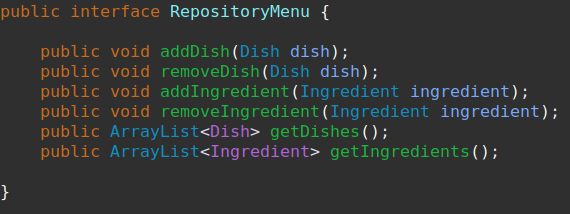
\includegraphics[width= 9cm]{"Codice/RepositoryMenu.PNG"}
\caption{Porzione di codice della classe RepositoryMenu}
\end{figure}

\newpage

\noindent ``FakeMenuData'' implementa ``RepositoryMenu'' ed \`e stato creato per avere un oggetto di storage fittizzio che ci permettesse di eseguire i test senza dover implementare sul momento piatti e ingredienti.

\begin{figure}[!h]
\centering
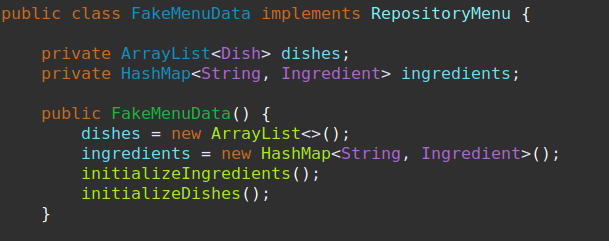
\includegraphics[width= 9cm]{"Codice/FakeMenuData1.PNG"}
\caption{Porzione di codice della classe FakeMenuData}
\end{figure}

\begin{figure}[!h]
\centering
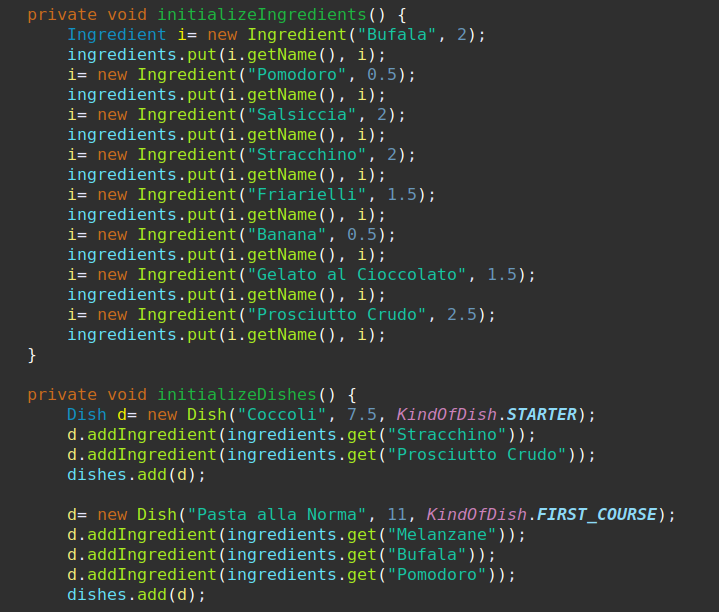
\includegraphics[width= 11cm]{"Codice/FakeMenuData2.PNG"}
\caption{Porzione di codice della classe FakeMenuData}
\end{figure}

\newpage

\subsection{Design Patterns}
\begin{comment}
Nella realizzazione del nostro progetto abbiamo ritenuto opportuno introdurre alcuni design patterns noti, indispensabili alla gestione di criticit\`a emerse durante il lavoro. I patterns utilizzati nel nostro applicativo sono: 
\\\\\\\
Nella realizzazione del nostro progetto ci siamo imbattuti in delle situazioni dove \`e emersa la necessit\`a di introdurre dei design patterns noti al fine di gestirle in modo agile ed elegante. I patterns utilizzati nel nostro applicativo sono:
\\\\\\
\end{comment}
All'interno del progetto abbiamo avuto la necessit\`a di introdurre alcuni design patterns noti per favorire la gestione di alcune dipendenze tra classi in modo agile ed elegante. I patterns utilizzati sono:

\begin{enumerate}
\item Observer
\item Singleton
\item MVC
\end{enumerate}

\subsubsection{Observer}
\label{Observer}
Il pattern comportamentale Observer \`e utilizzato per instaurare una relazione uno a molti fra oggetti cosicch\`e quando un oggetto cambia stato, tutte le sue dipendenze vengano informate e aggiornate automaticamente.\\
Nella nostra logica di dominio abbiamo avuto la necessit\`a di introdurre questo pattern per notificare alla cucina l'invio da parte del cameriere di una nuova comanda. Nonostante siano state deprecate, ci siamo serviti delle classi ``Observable'' e ``Observer'' e dei loro rispettivi metodi \textit{notifyObservers()} e \textit{update()} forniti dalla libreria java.util. Abbiamo inoltre deciso di implementare il pattern in modalit\`a push, la quale prevede che l'oggetto osservato notifichi gli osservatori inviando direttamente il cambiamento al momento della sua variazione. \\ Come \`e possibile infatti apprezzare dal Class Diagram di Figura \ref{ClassDiagram}, la classe ``OrderManager'' svolge il ruolo di oggetto osservato (``Observable'') che notifica l'arrivo di una nuova comanda inviandola direttamente alla cucina, alla pizzeria e al bar che svolgono il ruolo di osservatori (``Observer''). Questo avviene attraverso il metodo \textit{addOrder()} che preso come parametro il nuovo ordine piazzato dal cameriere lo invia agli ``Observers'' attraverso il metodo \textit{notifyObservers()}. Questi ultimi aggiorneranno poi il loro stato attraverso il metodo \textit{update()} (Vedi Sequence Diagram in Figura \ref{SequenceDiagram}).

\newpage

\subsubsection{Singleton}

Il pattern Creazionale Singleton \`e utilizzato per avere un'unica istanza di una determinata classe. \\
Nel nostro progetto abbiamo infatti introdotto questo pattern per garantire l'unicit\`a delle istanze delle classi ``TableContainer'', ``TableServiceContainer'' e ``OrderManager'', le quali interagiscono con pi\`u attori e classi e si ha quindi la necessit\`a che siano sempre le stesse. Come \`e possibile osservare nel Sequence Diagram di Figura \ref{SequenceDiagram}, gli attori non possiedono i riferimenti all'unica istanza di queste classi, ma li ottengono al momento che necessitano di utilizzarle attraverso il rispettivo metodo \textit{getInstance()}.

\subsubsection{MVC}

Il pattern Architetturale Model-View-Controller \`e utilizzato quando si ha la necessit\`a di accedere e modificare dei dati attraverso interazioni differenti con i client. Per far questo si possono dunque individuare le tre componenti principali:

\begin{itemize}
\item Model: \`E la parte che definisce il modello dei dati e le operazioni che possono essere  eseguite su queste presentandole alla View e al Controller. Il Model pu\`o inoltre notificare ai vari componenti della View eventuali aggiornamenti in seguito a richieste del Controller al fine di presentare ai Client dati sempre aggiornati.

\item View: Corrisponde alle varie interfacce dell'applicazione con cui gli utenti si possono trovare ad interagire per eseguire delle azioni sul sistema.
 
\item Controller: Svolge il ruolo da mediatore fra il View e il Model, trasformando le interazioni dell'utente sul primo in azioni sul secondo. Per farlo sfrutta inoltre un meccanismo che prende il nome di business logic. Questo consiste nel mettere in vita determinati oggetti del Model solo nel momento del loro effettivo bisogno, ossia quando devono interagire in risposta alle richieste del client.
\end{itemize}

\newpage

\noindent Nel nostro applicativo abbiamo sentito la necessit\`a di introdurre questo pattern in quanto i nostri attori interagiscono fra di loro e con il sistema al fine di scambiare dati e informazioni attraverso una molteplicit\`a di viste differenti. \\
Riportiamo quindi di seguito l'architettura del nostro applicativo suddivisa nelle tre componenti sopra descritte:

\begin{figure}[!h]
\centering
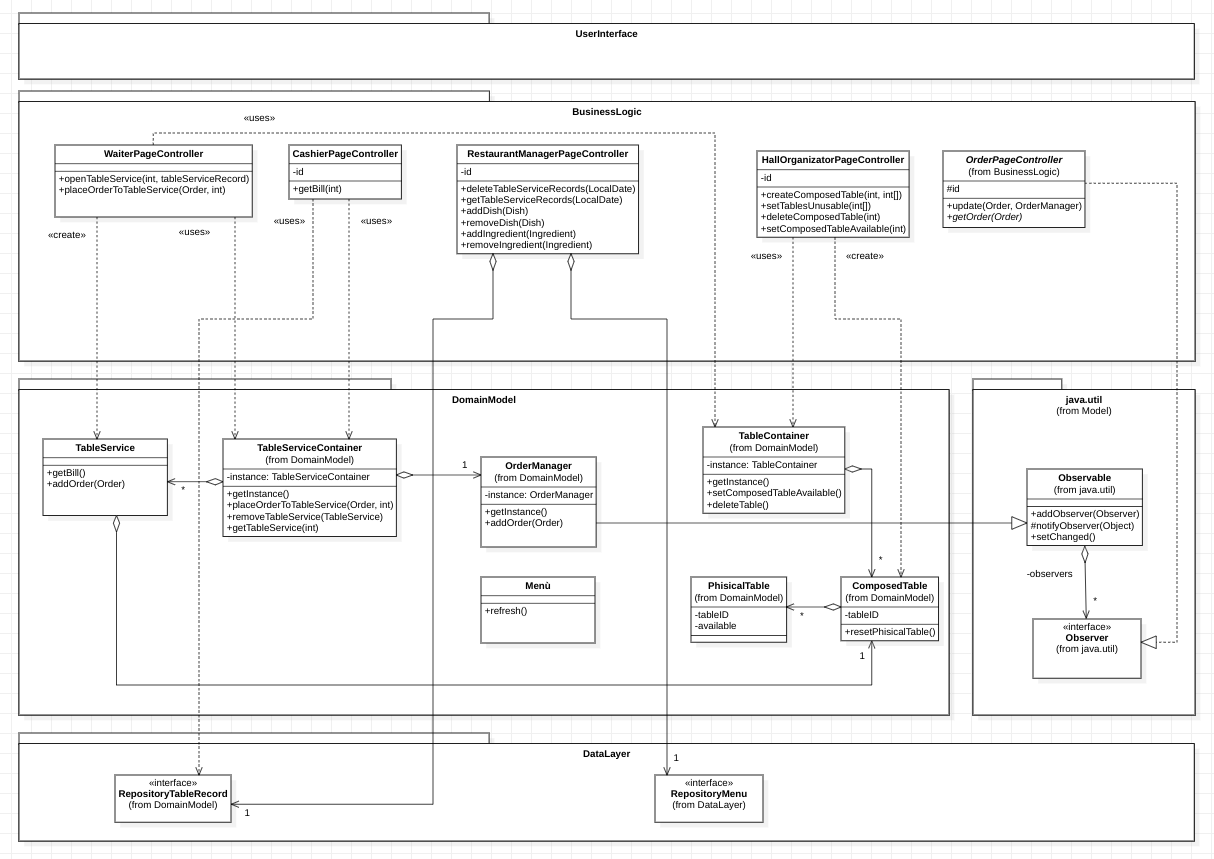
\includegraphics[width= 14cm]{"Immagini/Architecture.PNG"}
\caption{Raffigurazione dell'architettura dell'applicativo secondo lo schema Model-View-Controller}
\end{figure}

\newpage

\subsection{Disposizione delle classi nei package} 

\begin{figure}[!h]
\centering
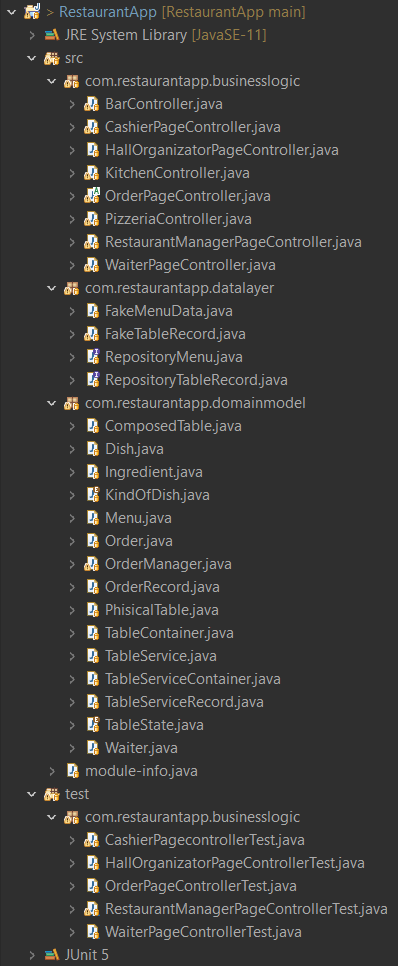
\includegraphics[width= 4.5cm]{"Immagini/Package.PNG"}
\caption{Raffigurazione della disposizione delle classi del progetto nei package}
\end{figure}

\newpage

\section{UnitTest}
Per testare la corretta interazione e collabborazione fra le parti abbiamo realizzato i seguenti test cases per alcune delle classi principali dell’applicativo: \\
\newline
Nel progetto \`e stato utilizzato il framework JUnit 5.0.

\subsection{WaiterPageControllerTest}

Nella seguente classe di test, \`e stata testato il controller del cameriere. In particolare dopo aver istanziato alcuni tavoli composti, vengono testate le funzioni \textit{openTableService()} e \textit{placeOrderToTableService()}. Ci\`o che ci ha spinto a scegliere questo test, \`e stato il fatto questi metodi sono tra i pi\`u essenziali tra quelli che stanno dietro la logica dell’applicativo.

\begin{figure}[!h]
\centering
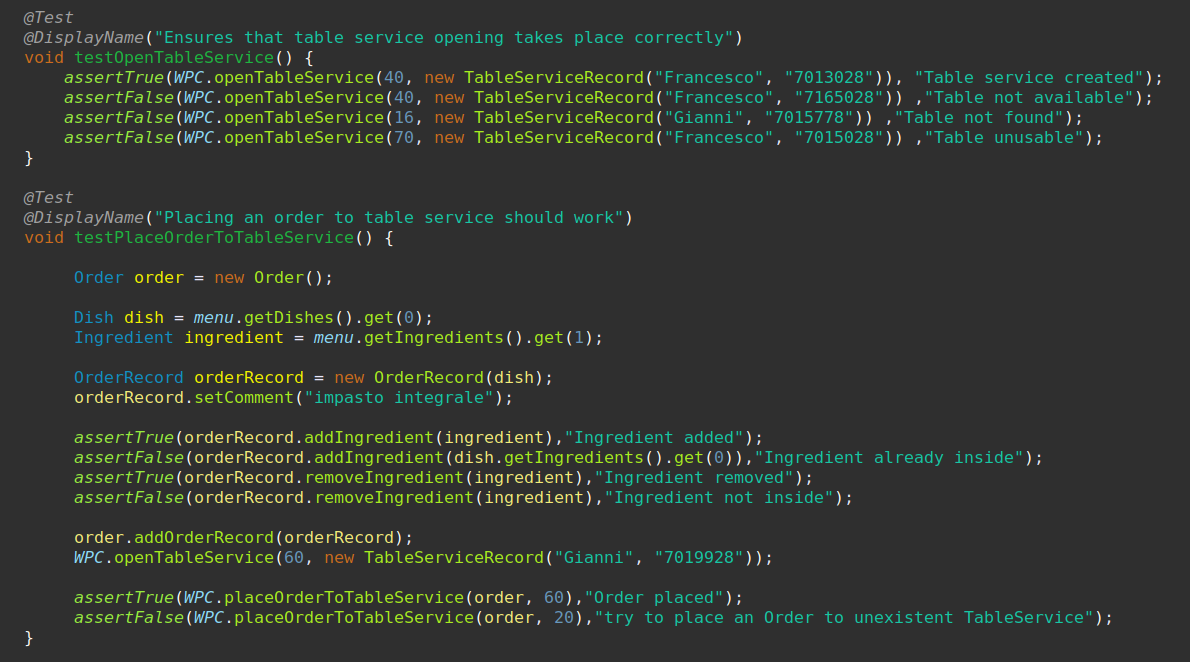
\includegraphics[width= 12cm]{"Codice/TestCameriere.PNG"}
\caption{Porzione di codice del test case del cameriere}
\end{figure}

\newpage

\subsection{RestaurantManagerPageControllerTest}

Il manager del ristorante pu\`o gestire sia i dati relativi ai clienti che il men\`u. Nella classe di test sottostante ci siamo concentrati sui metodi che visualizzano e cancellano i dati dei clienti. Gli altri metodi relativi al men\`u non li abbiamo testati per due ragioni principali: la prima \`e che non \`e presente un database sottostante implementato, la seconda \`e che sono analoghi ai precedenti.

\begin{figure}[!h]
\centering
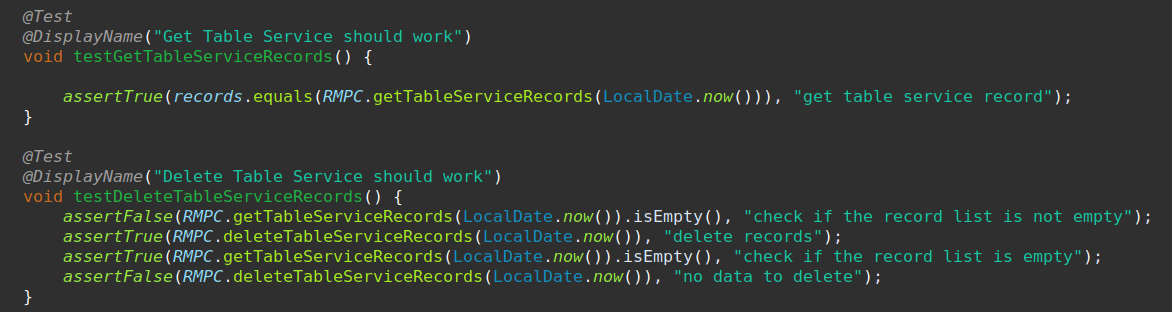
\includegraphics[width= 14cm]{"Codice/TestManager.PNG"}
\caption{Porzione di codice del test case del manager del ristorante}
\end{figure}

\subsection{CashierPageControllerTest}

Il controller del cassiere pu\`o calcolare il conto associato ad un servizio al tavolo. Nella classe di test sottostante è stato testato il corretto funzionamento del metodo \textit{getBill()}. In particolare vengono istanziati alcuni ordini associati a due diversi servizi al tavolo. Sono presenti piatti con ingredienti aggiunti e rimossi e ordini di storno. Quello che il cassiere deve controllare \`e che vengano calcolati i conti in modo corretto e che lo stato dei tavoli venga messo a ``DA PULIRE''.

\begin{figure}[!h]
\centering
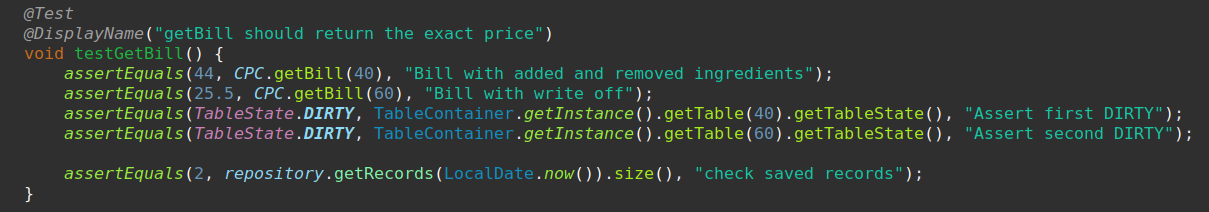
\includegraphics[width= 14cm]{"Codice/TestCashier.PNG"}
\caption{Porzione di codice del test case del cassiere}
\end{figure}

\newpage

\subsection{HallOrganizatorPageController}

Nella seguente classe di test, abbiamo testato tutti i metodi principali del controller dell’organizzatore della sala. In particolare dopo aver istanziato alcuni tavoli fisici, viene verificato il corretto funzionamento dei metodi \textit{createComposedTable(), deleteComposedTable(), setComposedTableAvailable()} e \textit{setTablesUnusable()}. La ragione che ci ha spinto ad effettuare questi test \`e, ancora una volta, il fatto che questi metodi sono tra i pi\`u essenziali tra quelli che stanno dietro la logica dell’applicativo.

\begin{figure}[!h]
\centering
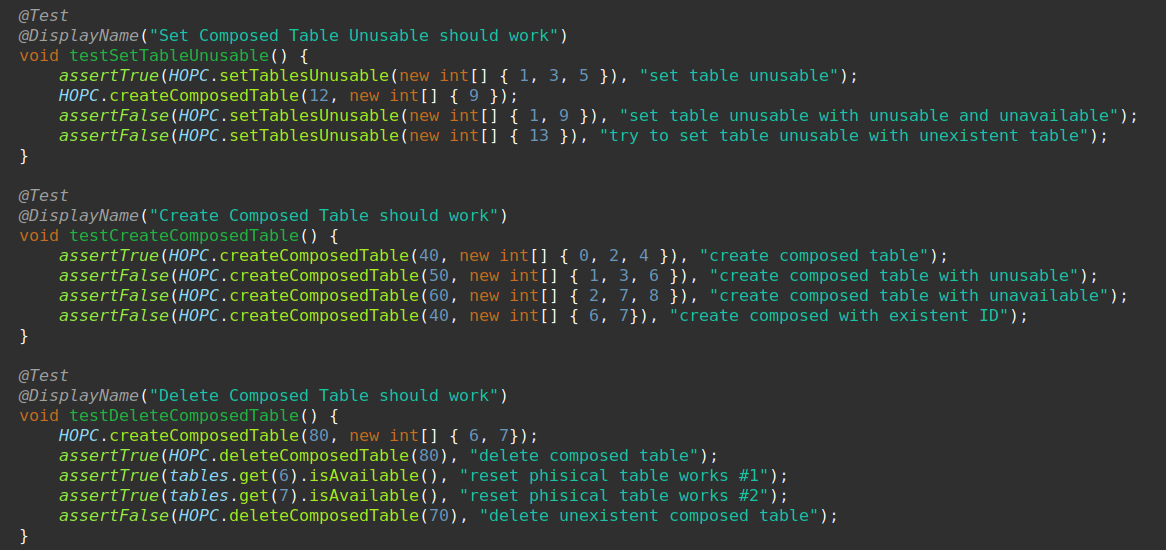
\includegraphics[width= 14cm]{"Codice/TestHall1.PNG"}
\caption{Porzione di codice del test case dell'organizzatore della sala}
\end{figure}

\begin{figure}[!h]
\centering
\includegraphics[width= 14cm]{"Codice/TestHall2.PNG"}
\caption{Porzione di codice del test case dell'organizzatore della sala}
\end{figure}

\newpage

\subsection{OrderPageControllerTest}

Nella seguente classe di test viene testato il corretto funzionamento del pattern Observer. In particolare vengono creati due ordini, di cui uno di storno, che vengono piazzati da un cameriere su un servizio al tavolo. Il test va a controllare che i controller della cucina, della pizzeria e del ristorante siano stati aggiornati correttamente. Successivamente viene piazzato un ulteriore ordine per controllare che i controller vengano aggiornati nel modo giusto.

\begin{figure}[!h]
\centering
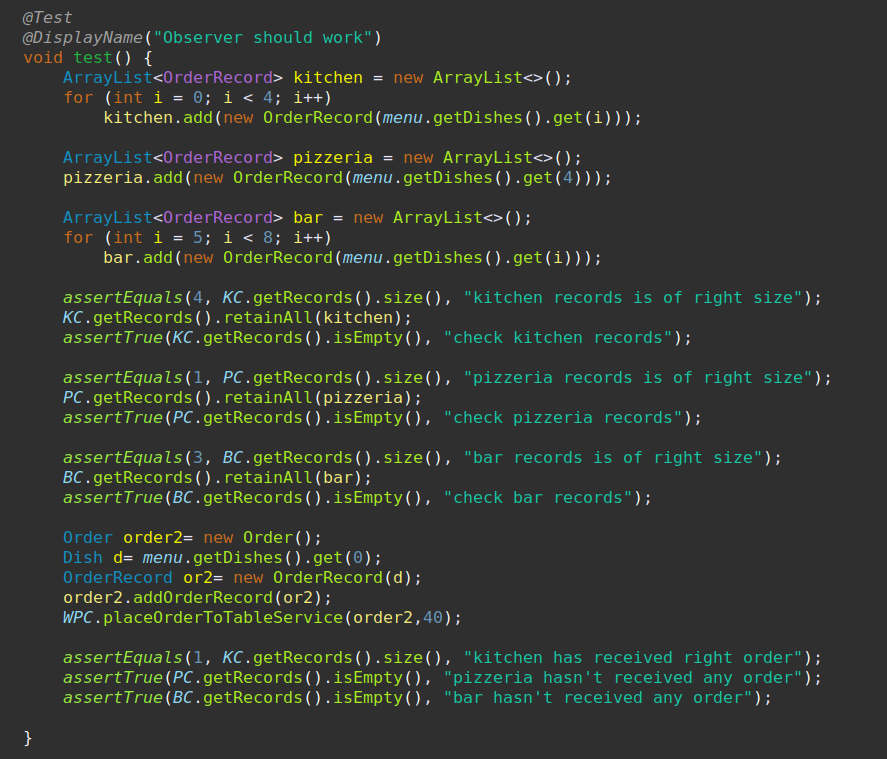
\includegraphics[width= 10cm]{"Codice/TestOrder.PNG"}
\caption{Porzione di codice del test case della cucina}
\end{figure}

\newpage

\section{Sequence Diagram}
Di seguito riportiamo un possibile scenario di interazione dei nostri attori:

\begin{figure}[!h]
\centering
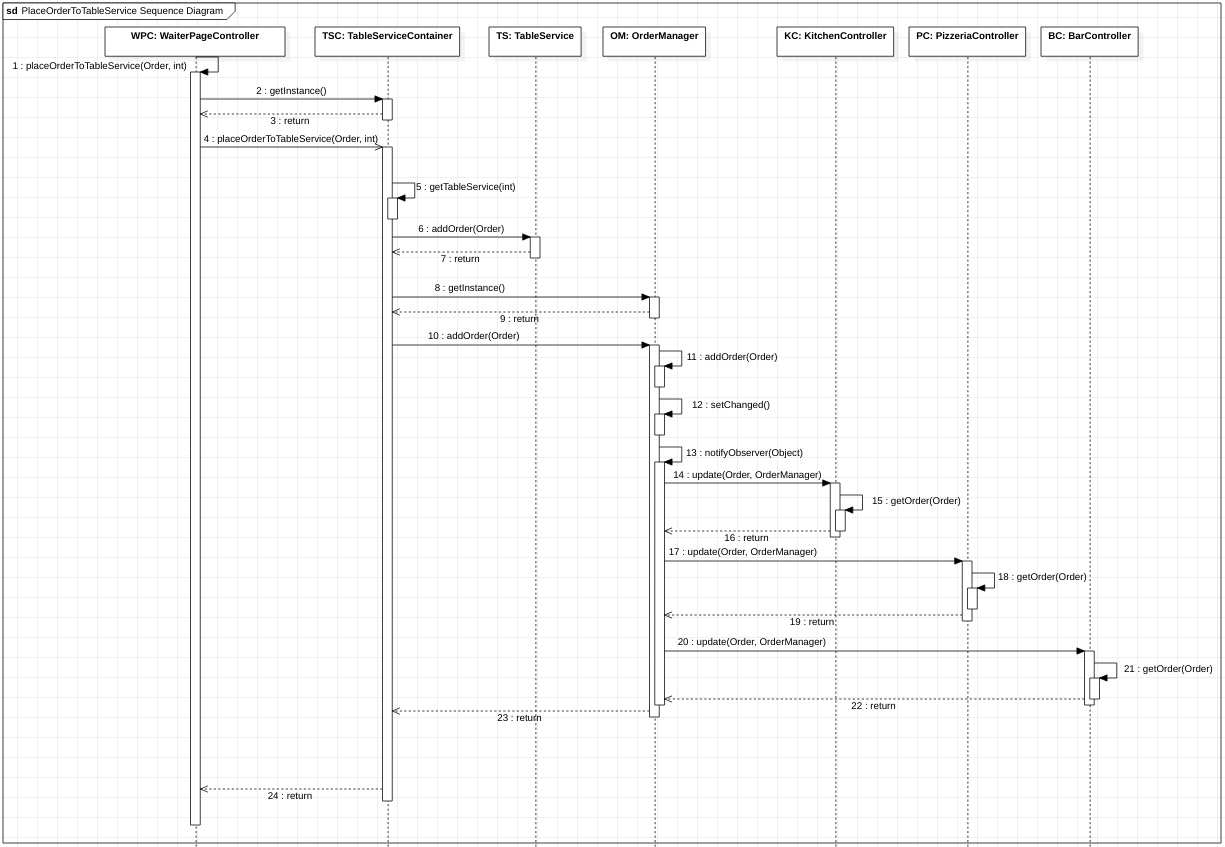
\includegraphics[width= 15cm]{"Immagini/SequenceDiagram.PNG"}
\caption{Sequence Diagram che documenta il flusso del controllo nel momento in cui il cameriere piazza un nuovo ordine a un tavolo}
\label{SequenceDiagram}
\end{figure}

\end{document}